% Generated by Sphinx.
\def\sphinxdocclass{report}
\documentclass[letterpaper,10pt,english]{sphinxmanual}
\usepackage[utf8]{inputenc}
\DeclareUnicodeCharacter{00A0}{\nobreakspace}
\usepackage[T1]{fontenc}
\usepackage{babel}
\usepackage{times}
\usepackage[Bjarne]{fncychap}
\usepackage{longtable}
\usepackage{sphinx}
\usepackage{multirow}


\title{pyicoteo Documentation}
\date{May 02, 2013}
\release{2.0.3}
\author{Juan González-Vallinas}
\newcommand{\sphinxlogo}{}
\renewcommand{\releasename}{Release}
\makeindex

\makeatletter
\def\PYG@reset{\let\PYG@it=\relax \let\PYG@bf=\relax%
    \let\PYG@ul=\relax \let\PYG@tc=\relax%
    \let\PYG@bc=\relax \let\PYG@ff=\relax}
\def\PYG@tok#1{\csname PYG@tok@#1\endcsname}
\def\PYG@toks#1+{\ifx\relax#1\empty\else%
    \PYG@tok{#1}\expandafter\PYG@toks\fi}
\def\PYG@do#1{\PYG@bc{\PYG@tc{\PYG@ul{%
    \PYG@it{\PYG@bf{\PYG@ff{#1}}}}}}}
\def\PYG#1#2{\PYG@reset\PYG@toks#1+\relax+\PYG@do{#2}}

\expandafter\def\csname PYG@tok@gd\endcsname{\def\PYG@tc##1{\textcolor[rgb]{0.63,0.00,0.00}{##1}}}
\expandafter\def\csname PYG@tok@gu\endcsname{\let\PYG@bf=\textbf\def\PYG@tc##1{\textcolor[rgb]{0.50,0.00,0.50}{##1}}}
\expandafter\def\csname PYG@tok@gt\endcsname{\def\PYG@tc##1{\textcolor[rgb]{0.00,0.27,0.87}{##1}}}
\expandafter\def\csname PYG@tok@gs\endcsname{\let\PYG@bf=\textbf}
\expandafter\def\csname PYG@tok@gr\endcsname{\def\PYG@tc##1{\textcolor[rgb]{1.00,0.00,0.00}{##1}}}
\expandafter\def\csname PYG@tok@cm\endcsname{\let\PYG@it=\textit\def\PYG@tc##1{\textcolor[rgb]{0.25,0.50,0.56}{##1}}}
\expandafter\def\csname PYG@tok@vg\endcsname{\def\PYG@tc##1{\textcolor[rgb]{0.73,0.38,0.84}{##1}}}
\expandafter\def\csname PYG@tok@m\endcsname{\def\PYG@tc##1{\textcolor[rgb]{0.13,0.50,0.31}{##1}}}
\expandafter\def\csname PYG@tok@mh\endcsname{\def\PYG@tc##1{\textcolor[rgb]{0.13,0.50,0.31}{##1}}}
\expandafter\def\csname PYG@tok@cs\endcsname{\def\PYG@tc##1{\textcolor[rgb]{0.25,0.50,0.56}{##1}}\def\PYG@bc##1{\setlength{\fboxsep}{0pt}\colorbox[rgb]{1.00,0.94,0.94}{\strut ##1}}}
\expandafter\def\csname PYG@tok@ge\endcsname{\let\PYG@it=\textit}
\expandafter\def\csname PYG@tok@vc\endcsname{\def\PYG@tc##1{\textcolor[rgb]{0.73,0.38,0.84}{##1}}}
\expandafter\def\csname PYG@tok@il\endcsname{\def\PYG@tc##1{\textcolor[rgb]{0.13,0.50,0.31}{##1}}}
\expandafter\def\csname PYG@tok@go\endcsname{\def\PYG@tc##1{\textcolor[rgb]{0.20,0.20,0.20}{##1}}}
\expandafter\def\csname PYG@tok@cp\endcsname{\def\PYG@tc##1{\textcolor[rgb]{0.00,0.44,0.13}{##1}}}
\expandafter\def\csname PYG@tok@gi\endcsname{\def\PYG@tc##1{\textcolor[rgb]{0.00,0.63,0.00}{##1}}}
\expandafter\def\csname PYG@tok@gh\endcsname{\let\PYG@bf=\textbf\def\PYG@tc##1{\textcolor[rgb]{0.00,0.00,0.50}{##1}}}
\expandafter\def\csname PYG@tok@ni\endcsname{\let\PYG@bf=\textbf\def\PYG@tc##1{\textcolor[rgb]{0.84,0.33,0.22}{##1}}}
\expandafter\def\csname PYG@tok@nl\endcsname{\let\PYG@bf=\textbf\def\PYG@tc##1{\textcolor[rgb]{0.00,0.13,0.44}{##1}}}
\expandafter\def\csname PYG@tok@nn\endcsname{\let\PYG@bf=\textbf\def\PYG@tc##1{\textcolor[rgb]{0.05,0.52,0.71}{##1}}}
\expandafter\def\csname PYG@tok@no\endcsname{\def\PYG@tc##1{\textcolor[rgb]{0.38,0.68,0.84}{##1}}}
\expandafter\def\csname PYG@tok@na\endcsname{\def\PYG@tc##1{\textcolor[rgb]{0.25,0.44,0.63}{##1}}}
\expandafter\def\csname PYG@tok@nb\endcsname{\def\PYG@tc##1{\textcolor[rgb]{0.00,0.44,0.13}{##1}}}
\expandafter\def\csname PYG@tok@nc\endcsname{\let\PYG@bf=\textbf\def\PYG@tc##1{\textcolor[rgb]{0.05,0.52,0.71}{##1}}}
\expandafter\def\csname PYG@tok@nd\endcsname{\let\PYG@bf=\textbf\def\PYG@tc##1{\textcolor[rgb]{0.33,0.33,0.33}{##1}}}
\expandafter\def\csname PYG@tok@ne\endcsname{\def\PYG@tc##1{\textcolor[rgb]{0.00,0.44,0.13}{##1}}}
\expandafter\def\csname PYG@tok@nf\endcsname{\def\PYG@tc##1{\textcolor[rgb]{0.02,0.16,0.49}{##1}}}
\expandafter\def\csname PYG@tok@si\endcsname{\let\PYG@it=\textit\def\PYG@tc##1{\textcolor[rgb]{0.44,0.63,0.82}{##1}}}
\expandafter\def\csname PYG@tok@s2\endcsname{\def\PYG@tc##1{\textcolor[rgb]{0.25,0.44,0.63}{##1}}}
\expandafter\def\csname PYG@tok@vi\endcsname{\def\PYG@tc##1{\textcolor[rgb]{0.73,0.38,0.84}{##1}}}
\expandafter\def\csname PYG@tok@nt\endcsname{\let\PYG@bf=\textbf\def\PYG@tc##1{\textcolor[rgb]{0.02,0.16,0.45}{##1}}}
\expandafter\def\csname PYG@tok@nv\endcsname{\def\PYG@tc##1{\textcolor[rgb]{0.73,0.38,0.84}{##1}}}
\expandafter\def\csname PYG@tok@s1\endcsname{\def\PYG@tc##1{\textcolor[rgb]{0.25,0.44,0.63}{##1}}}
\expandafter\def\csname PYG@tok@gp\endcsname{\let\PYG@bf=\textbf\def\PYG@tc##1{\textcolor[rgb]{0.78,0.36,0.04}{##1}}}
\expandafter\def\csname PYG@tok@sh\endcsname{\def\PYG@tc##1{\textcolor[rgb]{0.25,0.44,0.63}{##1}}}
\expandafter\def\csname PYG@tok@ow\endcsname{\let\PYG@bf=\textbf\def\PYG@tc##1{\textcolor[rgb]{0.00,0.44,0.13}{##1}}}
\expandafter\def\csname PYG@tok@sx\endcsname{\def\PYG@tc##1{\textcolor[rgb]{0.78,0.36,0.04}{##1}}}
\expandafter\def\csname PYG@tok@bp\endcsname{\def\PYG@tc##1{\textcolor[rgb]{0.00,0.44,0.13}{##1}}}
\expandafter\def\csname PYG@tok@c1\endcsname{\let\PYG@it=\textit\def\PYG@tc##1{\textcolor[rgb]{0.25,0.50,0.56}{##1}}}
\expandafter\def\csname PYG@tok@kc\endcsname{\let\PYG@bf=\textbf\def\PYG@tc##1{\textcolor[rgb]{0.00,0.44,0.13}{##1}}}
\expandafter\def\csname PYG@tok@c\endcsname{\let\PYG@it=\textit\def\PYG@tc##1{\textcolor[rgb]{0.25,0.50,0.56}{##1}}}
\expandafter\def\csname PYG@tok@mf\endcsname{\def\PYG@tc##1{\textcolor[rgb]{0.13,0.50,0.31}{##1}}}
\expandafter\def\csname PYG@tok@err\endcsname{\def\PYG@bc##1{\setlength{\fboxsep}{0pt}\fcolorbox[rgb]{1.00,0.00,0.00}{1,1,1}{\strut ##1}}}
\expandafter\def\csname PYG@tok@kd\endcsname{\let\PYG@bf=\textbf\def\PYG@tc##1{\textcolor[rgb]{0.00,0.44,0.13}{##1}}}
\expandafter\def\csname PYG@tok@ss\endcsname{\def\PYG@tc##1{\textcolor[rgb]{0.32,0.47,0.09}{##1}}}
\expandafter\def\csname PYG@tok@sr\endcsname{\def\PYG@tc##1{\textcolor[rgb]{0.14,0.33,0.53}{##1}}}
\expandafter\def\csname PYG@tok@mo\endcsname{\def\PYG@tc##1{\textcolor[rgb]{0.13,0.50,0.31}{##1}}}
\expandafter\def\csname PYG@tok@mi\endcsname{\def\PYG@tc##1{\textcolor[rgb]{0.13,0.50,0.31}{##1}}}
\expandafter\def\csname PYG@tok@kn\endcsname{\let\PYG@bf=\textbf\def\PYG@tc##1{\textcolor[rgb]{0.00,0.44,0.13}{##1}}}
\expandafter\def\csname PYG@tok@o\endcsname{\def\PYG@tc##1{\textcolor[rgb]{0.40,0.40,0.40}{##1}}}
\expandafter\def\csname PYG@tok@kr\endcsname{\let\PYG@bf=\textbf\def\PYG@tc##1{\textcolor[rgb]{0.00,0.44,0.13}{##1}}}
\expandafter\def\csname PYG@tok@s\endcsname{\def\PYG@tc##1{\textcolor[rgb]{0.25,0.44,0.63}{##1}}}
\expandafter\def\csname PYG@tok@kp\endcsname{\def\PYG@tc##1{\textcolor[rgb]{0.00,0.44,0.13}{##1}}}
\expandafter\def\csname PYG@tok@w\endcsname{\def\PYG@tc##1{\textcolor[rgb]{0.73,0.73,0.73}{##1}}}
\expandafter\def\csname PYG@tok@kt\endcsname{\def\PYG@tc##1{\textcolor[rgb]{0.56,0.13,0.00}{##1}}}
\expandafter\def\csname PYG@tok@sc\endcsname{\def\PYG@tc##1{\textcolor[rgb]{0.25,0.44,0.63}{##1}}}
\expandafter\def\csname PYG@tok@sb\endcsname{\def\PYG@tc##1{\textcolor[rgb]{0.25,0.44,0.63}{##1}}}
\expandafter\def\csname PYG@tok@k\endcsname{\let\PYG@bf=\textbf\def\PYG@tc##1{\textcolor[rgb]{0.00,0.44,0.13}{##1}}}
\expandafter\def\csname PYG@tok@se\endcsname{\let\PYG@bf=\textbf\def\PYG@tc##1{\textcolor[rgb]{0.25,0.44,0.63}{##1}}}
\expandafter\def\csname PYG@tok@sd\endcsname{\let\PYG@it=\textit\def\PYG@tc##1{\textcolor[rgb]{0.25,0.44,0.63}{##1}}}

\def\PYGZbs{\char`\\}
\def\PYGZus{\char`\_}
\def\PYGZob{\char`\{}
\def\PYGZcb{\char`\}}
\def\PYGZca{\char`\^}
\def\PYGZam{\char`\&}
\def\PYGZlt{\char`\<}
\def\PYGZgt{\char`\>}
\def\PYGZsh{\char`\#}
\def\PYGZpc{\char`\%}
\def\PYGZdl{\char`\$}
\def\PYGZhy{\char`\-}
\def\PYGZsq{\char`\'}
\def\PYGZdq{\char`\"}
\def\PYGZti{\char`\~}
% for compatibility with earlier versions
\def\PYGZat{@}
\def\PYGZlb{[}
\def\PYGZrb{]}
\makeatother

\begin{document}

\maketitle
\tableofcontents
\phantomsection\label{index::doc}


Pyicoteo* is a suite of tools for the analysis of high-throughput sequencing data. It works with genomic coordinates, it was mainly developed using Solexa/Illumina mapped reads, but it it's core is platform-agnostic. There are currently 6 different tools (5 command-line based, one configuration file based) and a python library for scripting:

\begin{Verbatim}[commandchars=\\\{\}]
* Pronounced as in Spanish  "picoteo"\_ /pɪkɒtɛɒ/:
  (n) Appetizer-type foods that accompany drinks before or instead of a meal.
\end{Verbatim}

If you have any problems or suggestions please join the \href{http://groups.google.com/group/pyicos}{Pyicoteo Google Group} and ask!


\chapter{Getting Started}
\label{index:welcome-to-pyicoteo}\label{index:getting-started}\label{index:pyicoteo-google-group}

\section{Download \& Install}
\label{index:download-install}
\textbf{Download Pyicoteo}  \href{https://bitbucket.org/regulatorygenomicsupf/pyicoteo/downloads}{Latest version} from our repository.

You can also download older versions (up to 1.1b) from our \href{http://sourceforge.net/projects/pyicos/}{Sourceforge repository}.

The command line tools can be used directly without installation. However, installation is recommended, and necessary if you intend to use the Pyicoteolib. To do so decompress the folder and run the setup.py script with administrator privileges:

\begin{Verbatim}[commandchars=\\\{\}]
python setup.py install
\end{Verbatim}


\section{Check installation}
\label{index:check-installation}
To test that the software was installed correctly, start a python console and try importing it by typing:

\begin{Verbatim}[commandchars=\\\{\}]
python
\textgreater{}\textgreater{}\textgreater{} import pyicoteolib
\textgreater{}\textgreater{}\textgreater{} import pyicoteolib.core
\end{Verbatim}

Also, you should find the tools in your command line.

\emph{Tip: If you are in a GNU/Linux system, type ``pyico'' in the command line and tap TAB twice. You should see something like this}:

\begin{Verbatim}[commandchars=\\\{\}]
pyicoclip        pyicoller        pyicos
pyicoenrich      pyicoregion      pyicotrocol
\end{Verbatim}


\section{Dependencies}
\label{index:dependencies}
In order to make it simple for the community, Pyicoteo basic functionality has no dependencies other than Python 2.6 or higher. However, there are 2 optional libraries you could install.


\subsection{Matplotlib}
\label{index:matplotlib}
For plotting capabilities, it is neccesary to install Matplotlib (\textgreater{} 1.0).


\subsection{Samtools}
\label{index:samtools}
Also, for BAM reading, while we offer a native python implementation, you can ask Pyicoteo to read BAM using samtools with the flag \code{-{-}samtools}.
Pyicoteo is not compatible with Python 3.


\section{The bedpk format}
\label{index:the-bedpk-format}
Some Pyicoteo tools (Pyicos, Pyicaller and Pyicoclip) default experiment and output formats is a derivative of UCSC \href{http://genome.ucsc.edu/FAQ/FAQformat.html\#format1}{Bed format} called bedpk. It follows the same starting fields ``chromosome/tag start end'' but it uses some of the original optional fields to include extra information. It is a cluster oriented format that aims to recollect information of a cluster of reads in a single comprehensive line.
\begin{figure}[htbp]
\centering
\capstart

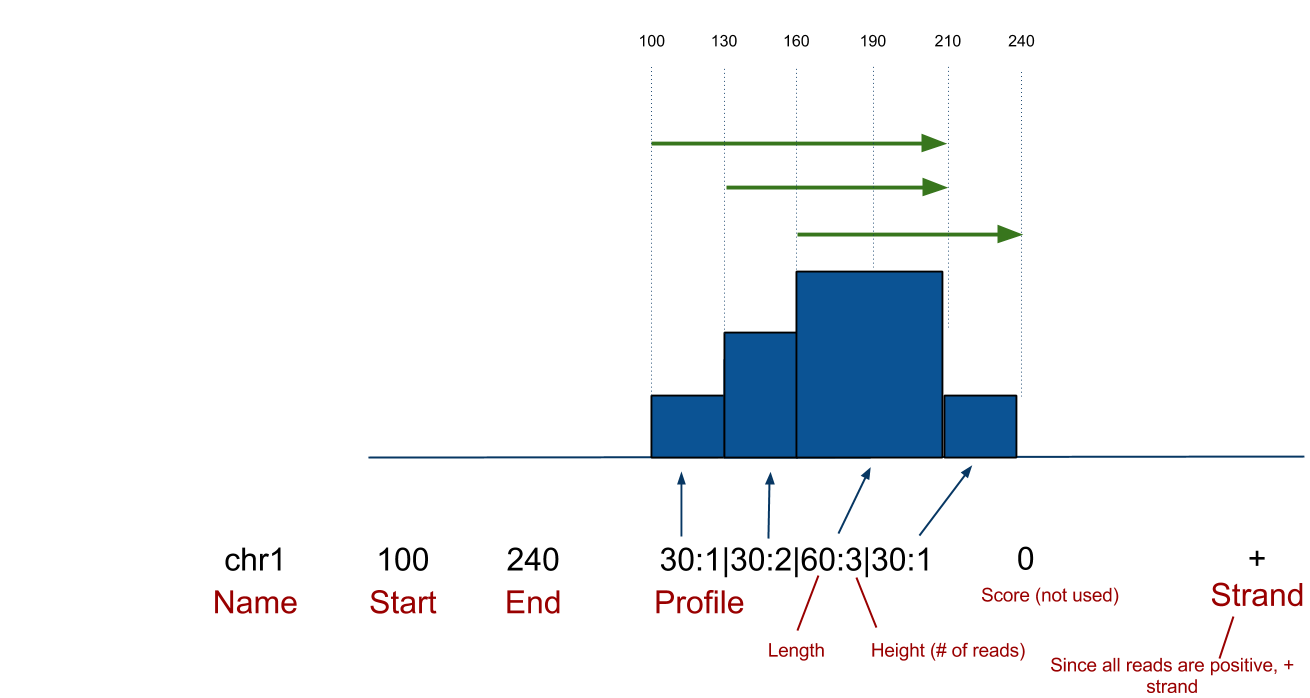
\includegraphics[width=50em]{bedpk_format.svg.png}
\caption{The bedpk format specification. It is exactly like a BED6 format, but using the 4th column to store extra information about how the cluster was built.}\end{figure}


\subsection{bedpk Column definition}
\label{index:bedpk-column-definition}\begin{enumerate}
\item {} 
Chromosome

\item {} 
Start coordinate

\item {} 
End coordinate

\item {} 
Profile: This field summarizes the accumulation of reads per nucleotide of the cluster. The first number is the number of bases covered, while the second will be the number of reads in those bases. See the example above

\item {} 
Height: The maximum height of the cluster. In this case, 3.

\item {} 
Strand: if ALL reads that  are positive strand \code{+}, if they are all negative \code{-}. Otherwise \code{.}

\item {} 
Summit: The position where the maximum height is found. The binding site is expected to be close to the summit.

\item {} 
Area: The area covered by the cluster.

\item {} 
p-value: The significance of the cluster calculated by the poisson operation based on peak heights or numbers of reads.

\end{enumerate}


\chapter{Pyicoteolib}
\label{index:pyicoteolib}
A python library that is the building blocks of all the other tools and a useful tool for python scripting.

Read more about it at:


\section{Pyicoteolib.core}
\label{pyicoteolib:pyicoteolib-core}\label{pyicoteolib::doc}\label{pyicoteolib:libdocs}
Pyicoteolib is the library and the building blocks of the Pyicoteo suite. The pyicoteolib.core library contains the main holders of data in the


\subsection{ReadCluster}
\label{pyicoteolib:readcluster}
A ReadCluster object may contain one read or a group of \textbf{overlapping} reads. It can read both tag like (bed, sam, bam..) and histogram like (wig, bed\_pk...) formats. Instances of the ReadCluster object can be added, compared, subtracted to other readCluster objects with standard python syntax.

The ReadCluster object is optimized in order to deal with millions of overlaps, and has been tested with multiple different HTS datasets. The optimization consists in 2 main principles:


\subsubsection{Common python operators}
\label{pyicoteolib:common-python-operators}
All the following standard operators are supported:


\paragraph{Adding}
\label{pyicoteolib:adding}
Adding combines the signal of 2 different ReadClusters, with nucleotide precision:

\begin{Verbatim}[commandchars=\\\{\}]
cluster1 = ReadCluster(read=PK)
cluster2 = ReadCluster(read=PK)
cluster1.read\_line('chr1 1 45 9:2.00\textbar{}41:3.00\textbar{}50:2.00\textbar{}45:1.00')
cluster2.read\_line('chr1 1 125 9:4.00\textbar{}41:3.00\textbar{}30:2.00\textbar{}45:1.00')
result = cluster1 + cluster2

result.write\_line()

        chr1    1       145     50:6.00\textbar{}30:4.00\textbar{}20:3.00\textbar{}25:2.00\textbar{}20:1.00 6.0     .       25      550.0
\end{Verbatim}


\paragraph{Subtracting}
\label{pyicoteolib:subtracting}
Substracts the signal of 2 different ReadClusters, with nucleotide precision:

\begin{Verbatim}[commandchars=\\\{\}]
\PYG{n}{cluster1} \PYG{o}{=} \PYG{n}{ReadCluster}\PYG{p}{(}\PYG{n}{read}\PYG{o}{=}\PYG{n}{SAM}\PYG{p}{)}
\PYG{n}{cluster2} \PYG{o}{=} \PYG{n}{ReadCluster}\PYG{p}{(}\PYG{n}{read}\PYG{o}{=}\PYG{n}{PK}\PYG{p}{)}
\PYG{n}{cluster1}\PYG{o}{.}\PYG{n}{read\PYGZus{}line}\PYG{p}{(}\PYG{l+s}{\PYGZsq{}}\PYG{l+s}{SL\PYGZhy{}XAJ\PYGZus{}1\PYGZus{}FC305HJAAXX:2:21:872:1402  0       chr1    1       50      36M     *       0       0       AAAAGGGGGAATAAAAAGTAACCCAAAACTAACTAT    \PYGZlt{}\PYGZlt{}\PYGZlt{},7\PYGZlt{}\PYGZlt{}\PYGZlt{}\PYGZlt{}\PYGZlt{}7\PYGZlt{}1:71)\PYGZlt{}+51\PYGZlt{}+\PYGZlt{}5(75()1344+2    PG:Z:FC\PYGZus{}305HJAAXX\PYGZus{}ln\PYGZus{}2.dat}\PYG{l+s}{\PYGZsq{}}\PYG{p}{)}
\PYG{n}{cluster2}\PYG{o}{.}\PYG{n}{read\PYGZus{}line}\PYG{p}{(}\PYG{l+s}{\PYGZsq{}}\PYG{l+s}{chr1 1 125 9:4.00\textbar{}41:3.00\textbar{}30:2.00\textbar{}45:1.00}\PYG{l+s}{\PYGZsq{}}\PYG{p}{)}
\PYG{n}{result} \PYG{o}{=} \PYG{n}{cluster2} \PYG{o}{\PYGZhy{}} \PYG{n}{cluster1}

\PYG{n}{result}\PYG{o}{.}\PYG{n}{write\PYGZus{}line}\PYG{p}{(}\PYG{p}{)}
\end{Verbatim}


\paragraph{Length}
\label{pyicoteolib:length}
Returns the length of the read cluster:

\begin{Verbatim}[commandchars=\\\{\}]
\PYG{n}{c} \PYG{o}{=} \PYG{n}{Cluster}\PYG{p}{(}\PYG{n}{name}\PYG{o}{=}\PYG{l+s}{\PYGZdq{}}\PYG{l+s}{chrX}\PYG{l+s}{\PYGZdq{}}\PYG{p}{,} \PYG{n}{start}\PYG{o}{=}\PYG{l+m+mi}{1}\PYG{p}{,} \PYG{n}{end}\PYG{o}{=}\PYG{l+m+mi}{10000}\PYG{p}{)}
\PYG{n+nb}{len}\PYG{p}{(}\PYG{n}{c}\PYG{p}{)}

\PYG{l+m+mi}{10000}
\end{Verbatim}


\paragraph{Comparison operators (\textless{} \textgreater{} == !=)}
\label{pyicoteolib:comparison-operators}
This indicates which read cluster is before another in a chromosome:

\begin{Verbatim}[commandchars=\\\{\}]
\PYG{n}{c1} \PYG{o}{=} \PYG{n}{Cluster}\PYG{p}{(}\PYG{n}{name}\PYG{o}{=}\PYG{l+s}{\PYGZdq{}}\PYG{l+s}{chr1}\PYG{l+s}{\PYGZdq{}}\PYG{p}{,} \PYG{n}{start}\PYG{o}{=}\PYG{l+m+mi}{100}\PYG{p}{,} \PYG{n}{end}\PYG{o}{=}\PYG{l+m+mi}{1000}\PYG{p}{)}
\PYG{n}{c1\PYGZus{}copy} \PYG{o}{=} \PYG{n}{Cluster}\PYG{p}{(}\PYG{n}{name}\PYG{o}{=}\PYG{l+s}{\PYGZdq{}}\PYG{l+s}{chr1}\PYG{l+s}{\PYGZdq{}}\PYG{p}{,} \PYG{n}{start}\PYG{o}{=}\PYG{l+m+mi}{100}\PYG{p}{,} \PYG{n}{end}\PYG{o}{=}\PYG{l+m+mi}{1000}\PYG{p}{)}
\PYG{n}{c2} \PYG{o}{=} \PYG{n}{Cluster}\PYG{p}{(}\PYG{n}{name}\PYG{o}{=}\PYG{l+s}{\PYGZdq{}}\PYG{l+s}{chr1}\PYG{l+s}{\PYGZdq{}}\PYG{p}{,} \PYG{n}{start}\PYG{o}{=}\PYG{l+m+mi}{50000}\PYG{p}{,} \PYG{n}{end}\PYG{o}{=}\PYG{l+m+mi}{100000}\PYG{p}{)}

\PYG{n}{c1} \PYG{o}{\PYGZgt{}} \PYG{n}{c2}
\PYG{n+nb+bp}{False}
\PYG{n}{c1} \PYG{o}{==} \PYG{n}{c1\PYGZus{}copy}
\PYG{n+nb+bp}{True}
\end{Verbatim}

Lets see some usage examples.


\subsubsection{Read a .bed file, print the chromosome and the length of each read}
\label{pyicoteolib:read-a-bed-file-print-the-chromosome-and-the-length-of-each-read}
\begin{Verbatim}[commandchars=\\\{\}]
\PYG{k+kn}{from} \PYG{n+nn}{pyicoteolib.core} \PYG{k+kn}{import} \PYG{n}{ReadCluster}\PYG{p}{,} \PYG{n}{BED}

\PYG{n}{bed\PYGZus{}file} \PYG{o}{=} \PYG{n+nb}{open}\PYG{p}{(}\PYG{l+s}{\PYGZdq{}}\PYG{l+s}{/path/to/myfile.bed}\PYG{l+s}{\PYGZdq{}}\PYG{p}{)}

\PYG{k}{for} \PYG{n}{line} \PYG{o+ow}{in} \PYG{n}{bed\PYGZus{}file}\PYG{p}{:}
        \PYG{n}{rc} \PYG{o}{=} \PYG{n}{ReacCluster}\PYG{p}{(}\PYG{n}{read\PYGZus{}as}\PYG{o}{=}\PYG{n}{BED}\PYG{p}{)}
        \PYG{n}{rc}\PYG{o}{.}\PYG{n}{read\PYGZus{}line}\PYG{p}{(}\PYG{n}{l}\PYG{p}{)}
        \PYG{k}{print} \PYG{n+nb}{len}\PYG{p}{(}\PYG{n}{rc}\PYG{p}{)}\PYG{p}{,} \PYG{n}{rc}\PYG{o}{.}\PYG{n}{area}\PYG{p}{(}\PYG{p}{)}
\end{Verbatim}


\subsubsection{Read some .bed lines, cluster them, output a wiggle file}
\label{pyicoteolib:read-some-bed-lines-cluster-them-output-a-wiggle-file}\begin{quote}

cluster =  Cluster(read=BED)
cluster.read\_line(`chr1 1 20000 666 hola +')
cluster.read\_line(`chr1 1 20000 666 hola +')
cluster.read\_line(`chr1 1 20000 666 hola +')
cluster.read\_line(`chr1 1001 20000 666 hola +')
cluster.write\_line()
\end{quote}


\paragraph{ReadRegion}
\label{pyicoteolib:readregion}
A ReadRegion object holds a genomic region that may contain ReadClusters


\subsection{pyicoteolib.utils}
\label{pyicoteolib:pyicoteolib-utils}

\subsection{BAM reader}
\label{pyicoteolib:bam-reader}

\subsection{Credit}
\label{pyicoteolib:credit}\begin{itemize}
\item {} 
Developers: Juan González-Vallinas, Ferran Lloret

\item {} 
Unit and beta Testing: Juan González-Vallinas, Ferran Lloret

\item {} 
Supervision: Eduardo Eyras

\end{itemize}


\chapter{Command-line based tools}
\label{index:command-line-based-tools}

\section{pyicos command line operations}
\label{pyicos:pyicos-command-line-operations}\label{pyicos::doc}
Pyicos is a command line utility for the conversion and manipulation of genomic coordinates files. It follows a command/sub-command structure

In the interactive help you can visualize the available commands list:

\begin{Verbatim}[commandchars=\\\{\}]
\PYG{n}{pyicos} \PYG{o}{\PYGZhy{}}\PYG{n}{h}
\end{Verbatim}

If you are interested in the usage of a particular command (for example, `extend') and the meaning of its flags type:

\begin{Verbatim}[commandchars=\\\{\}]
pyicos extend -h
\end{Verbatim}

Here we explain briefly what each subcommand does and we give some examples:


\subsection{convert}
\label{pyicos:convert}
Converting a file from one format to another format. Currently supported format are:

experiment: Bed, Wiggle files (bed\_wiggle), SAM, BAM, Eland, bedpk (Pyicos default compressed format), bedspk (Pyicos stranded compressed format)

output: Bed, Wiggle files (bed\_wiggle, variable\_wiggle), SAM, BAM, Eland, bedpk (Pyicos default compressed format), bedspk (Pyicos stranded compressed format)

This operation is useful if you only want to convert your data to another format. Other operations already include a conversion if you specify different experiment and output formats.

Convert a bed file to a half-open variable wig file:

\begin{Verbatim}[commandchars=\\\{\}]
pyicos convert my\_experiment.bed my\_experiment.wig -f bed -F variable\_wig -O
\end{Verbatim}

Convert all pk files in a folder to bed wig files:

\begin{Verbatim}[commandchars=\\\{\}]
pyicos convert my\_experiment\_folder/ outputfolder/ -f pk -F bed\_wig
\end{Verbatim}


\subsection{remregions}
\label{pyicos:remregions}
Remove regions that overlap with the regions in the ``black list'' file.

Example:

\begin{Verbatim}[commandchars=\\\{\}]
pyicos remregions my\_experiment.bed regions.bed my\_result.bed --experiment-format bed --open-experiment --region-format bed --open-region --output-format bed --open-output
\end{Verbatim}


\subsection{remduplicates}
\label{pyicos:remduplicates}
Remove the duplicated reads in a file. A duplicate is a read with the same start position as a read that has already been seen. You can choose how many duplicates you want to tolerate. If you want to keep only one read for a start position, set the duplicates to 0.

Example:

Here we tolerate 1 duplicate so a read can not occur more often than twice:

\begin{Verbatim}[commandchars=\\\{\}]
pyicos remduplicates my\_experiment.bed my\_experiment\_1dupl.bed --duplicates 1 -f bed -o -F bed
\end{Verbatim}


\subsection{strcorr (Strand Correlation)}
\label{pyicos:strcorr-strand-correlation}
Finds the optimal extension value by finding the ``gap'' between groups of positive and negative cluster of reads by performing a pearson correlation test.


\subsection{extend}
\label{pyicos:extend}
Extend the reads to the estimated fragment length, taking into consideration if they map to the forward or reverse strand of the reference genome.
\begin{figure}[htbp]
\centering

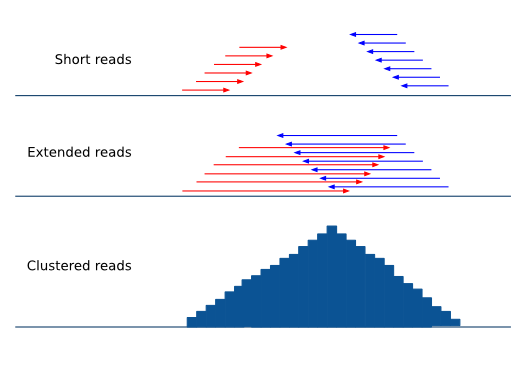
\includegraphics{Extend.png}
\end{figure}

Examples:

We have a bed file (half open) with reads between 30 and 50 nucleotides long. We want to extend them all to 150 nucleotides and write the output in bedpk-format to accelerate the successive operations:

\begin{Verbatim}[commandchars=\\\{\}]
pyicos extend my\_experiment.bed my\_experiment\_ext.bedpk 150 -f bed -o
\end{Verbatim}

We do the same with the control:

\begin{Verbatim}[commandchars=\\\{\}]
pyicos extend control.bed control\_ext.bedpk 150 -f bed -o
\end{Verbatim}

To visualize the data in a genome browser we set the output to be half-open bed\_wig:

\begin{Verbatim}[commandchars=\\\{\}]
pyicos extend my\_experiment.bed my\_experiment\_ext.bed\_wig 150 -f bed -o -F bed\_wig -O
\end{Verbatim}


\subsection{subtract}
\label{pyicos:subtract}
Subtract the reads in one file from the reads in another file. Using background data (control) improves the results because the background distribution is not supposed to be normal,
and statistical approaches to obtain this have a limited reach.

The most straightforward approach is to subtract the control from the sample. Make sure the sample has been \textbf{normalized} to the control beforehand!
Pyicos maintains a 1bp resolution by subtracting the reads nucleotide by nucleotide, rather than doing a statistical approximation.
Operating with directories will only give appropiate results if the files and the control are paired in alphabetical order.

Example:

Subtract the control from the experiment (both have already been extended, converted to bedpk and normalized):

\begin{Verbatim}[commandchars=\\\{\}]
pyicos subtract my\_experiment\_ext\_norm.bedpk control\_ext.bedpk my\_experiment\_ext\_norm\_subtr.bedpk
\end{Verbatim}


\subsection{split}
\label{pyicos:split}
Split peaks into subpeaks in case they fulfill the criteria.

Criteria: peak has at least two neighboring maxima between which the coverage of reads falls below the threshold. The threshold can be set by the user and it reflects a proportion of the lower maximum.

Output: bedpk or Wiggle files
\begin{figure}[htbp]
\centering

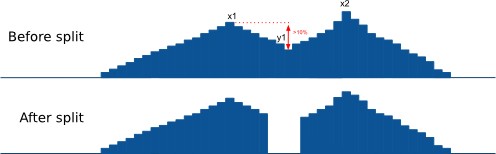
\includegraphics{Split.png}
\end{figure}

Example:

\begin{Verbatim}[commandchars=\\\{\}]
pyicos split peaks.bedpk peaks\_split.bedpk --split-proportion 0.9
\end{Verbatim}


\subsection{discard}
\label{pyicos:discard}
Discards peaks that look like artifacts due to the sequencing bias. Here we refer to peaks that look like blocks that result from duplicates (reads with the same start position).

Output: bedpk or Wiggle files
\begin{figure}[htbp]
\centering


\includegraphics{Artifact.png}
\end{figure}

Example:

\begin{Verbatim}[commandchars=\\\{\}]
pyicos discard peaks.bedpk peaks\_discA.bedpk
\end{Verbatim}


\subsection{poisson}
\label{pyicos:poisson}
This is the test to assess significance of peaks along the whole genome (as for ChIP-Seq). We do 3 different global poisson statistical tests for each chromosome in a file:
\begin{quote}

\textbf{Max height analysis}

Lambda is calculated from the maximum heights of the clusters by calculating the average height of a cluster in a given region. Pyicos will obtain the p-value\_height of one cluster having a height k by chance.

\textbf{Number of reads analysis}

Lambda is obtained from the number of reads in clusters.

\textbf{Nucleotide analysis}

Lambda is obtained from the number of nucleotides in a cluster.
\end{quote}

Example:

\begin{Verbatim}[commandchars=\\\{\}]
pyicos poisson peaks.bedpk
\end{Verbatim}


\subsection{filter}
\label{pyicos:filter}
Detect and select significant clusters in the file. There are two steps in this operation: Through the poisson operation the thresholds are determined. Next the peaks are filtered according to these thresholds.

Output: bedpk or Wiggle files
\begin{figure}[htbp]
\centering

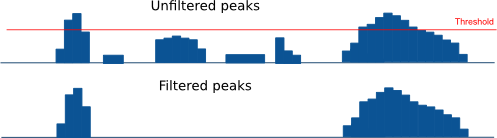
\includegraphics{Filter.png}
\end{figure}

Example:

\begin{Verbatim}[commandchars=\\\{\}]
pyicos filter peaks.bedpk significant\_peaks.bedpk 150
\end{Verbatim}


\subsection{push}
\label{pyicos:push}
Push the reads in the corresponding strand. If a read doesn't have a strand, it will be pushed from left to right.

This operation requires tag-like files (bed, eland, sam).

Example:

\begin{Verbatim}[commandchars=\\\{\}]
pyicos push my\_experiment.bed my\_experiment\_pushed100.bed 100 -f bed -F bed
\end{Verbatim}


\subsection{Credit}
\label{pyicos:credit}\begin{itemize}
\item {} 
Developer: Juan González-Vallinas

\item {} 
Beta Testing: Eneritz Agirre, Sonja Althammer, Juan González-Vallinas

\item {} 
Supervision: Eduardo Eyras

\end{itemize}


\section{Pyicoller}
\label{pyicoller:pyicoller}\label{pyicoller::doc}
This peak caller is a combinations of some of Pyicos commands (extend, normalize, subtract, remove, poisson and filter) for the task of calling peaks from a ChIP-Seq experiment (with narrow peaks). A control file is optional but recommended.

Example:

\begin{Verbatim}[commandchars=\\\{\}]
pyicoller my\_experiment.bed significant\_peaks.bedpk -f bed -o --control control.bed --control-format bed --open-control --region regions\_to\_be\_removed.bed --remlabels chrY --correction 0.8 --k-limit 20 --p-value 0.001 -x 130
\end{Verbatim}


\subsection{Credit}
\label{pyicoller:credit}\begin{itemize}
\item {} 
Developer: Juan González-Vallinas

\item {} 
Beta testing: Sonja Althammer, Eneritz Agirre, Nuria Conde Pueyo

\item {} 
Benchmarking against other peak callers: Sonja Althammer

\item {} 
Performance benchmarking: Juan González-Vallinas

\end{itemize}


\section{Pyicoenrich}
\label{pyicoenrich:pyicoenrich}\label{pyicoenrich::doc}

\subsection{Introduction}
\label{pyicoenrich:introduction}
Enrichment analysis can be applied on any type of -seq data. Pyicoenrich performs enrichment analysis on sequenced reads from two conditions. Like this you can find out how significant the difference of these two conditions is, in terms of the number/density of reads overlapping a region of interest.
\begin{figure}[htbp]
\centering

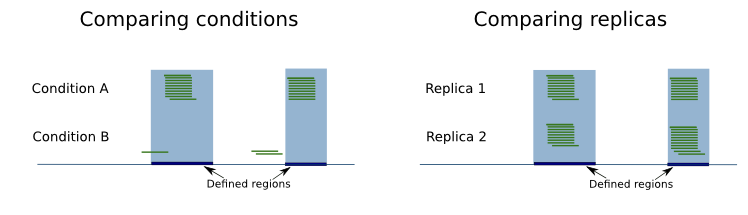
\includegraphics{enrichment.png}
\end{figure}


\subsection{MA Plot}
\label{pyicoenrich:ma-plot}
Pyicoenrich is based on the \href{http://en.wikipedia.org/wiki/MA\_plot}{MA-Plot}.

(Figura)


\subsection{Region exploration}
\label{pyicoenrich:region-exploration}
If a region file is provided, Pyicoenrich returns for each region a Z-Score (See counts file description) which indicates the enrichment/depletion of condition A over condition B. If no region file is provided, Pyicoenrich provides the options to take the union of reads from both conditions as a region and gives back Z-Scores for the generated regions. As regions with 0 reads in one condition might be especially interesting.

In order to decide what regions are to be explored, you have 3 main options:


\subsubsection{Generate a file with the --region-magic flag and GTF file}
\label{pyicoenrich:generate-a-file-with-the-region-magic-flag-and-gtf-file}
See {\hyperref[pyicoregion:pyicoregiondocs]{\emph{Pyicoregion}}} for examples on how to use \code{-{-}region-magic} flag to automatically explore exons, introns and the whole genome using sliding windows automatically from GTF files.


\subsubsection{Provide a regions file}
\label{pyicoenrich:provide-a-regions-file}
If a region file is provided, Pyicoenrich returns for each region a z-Score (among others) which indicates the enrichment/depletion of condition A over condition B. The region file should be in BED format. Also, you may consider only discontinuous regions by using the BED12 format:

\begin{Verbatim}[commandchars=\\\{\}]
pyicoenrich -reads kidney1.bed liver1.bed -output Pyicoenrich\_Kidney\_Liver\_result\_Counts -f bed --region genes.bed
\end{Verbatim}


\subsubsection{Do nothing}
\label{pyicoenrich:do-nothing}
Don't really know where you want to look yet? If no region file is provided, Pyicoenrich will automatically generate one with taking he union of reads from both conditions as a region and gives back Z-Scores for the generated regions.

The flag \code{-{-}proximity} controls the distance with which the regions are considered ``joined''. Default is 50nt:

\begin{Verbatim}[commandchars=\\\{\}]
pyicoenrich -reads kidney1.bed liver1.bed -output Pyicoenrich\_Kidney\_Liver\_result -f bed --proximity 50nt
\end{Verbatim}
\begin{figure}[htbp]
\centering

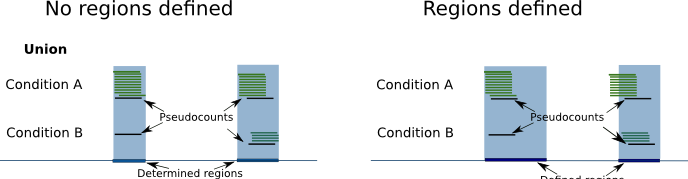
\includegraphics{region_definition.png}
\end{figure}


\subsection{\texttt{-{-}pseudocounts} flag}
\label{pyicoenrich:pseudocounts-flag}
As regions with 0 reads in one condition might be especially interesting, Pyicoenrich can use pseudocounts, in order to avoid a division by 0: Pyicoenrich calculates the ratio of number of reads in both conditions. As there might not be any reads in a region, Pyicoenrich assumes that there is already 1 read in each region in each condition.


\subsection{\texttt{-{-}stranded} flag}
\label{pyicoenrich:stranded-flag}

\subsection{Replica or technical control (swap)}
\label{pyicoenrich:replica-or-technical-control-swap}
To calculate the Z-Score, Pyicoenrich compares the differences between condition A and condition B with the differences between A and A' (while A' is the biological replica of A). If no biological replica is available, Pyicoenrich uses a sample swap as a reference. With sample swap we mean that reads from condition A and B are mixed randomly and divided in two sets (with size of those of A and B). In the two resulting sets we do not expect any significant differences, just like in replicas.
\begin{figure}[htbp]
\centering
\capstart

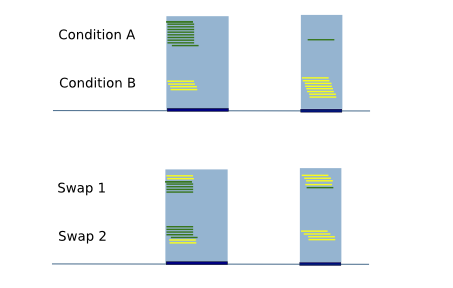
\includegraphics{swap.png}
\caption{Technical replica (swap) illustration}\end{figure}


\subsubsection{Examples}
\label{pyicoenrich:examples}
With replica:

\begin{Verbatim}[commandchars=\\\{\}]
pyicoenrich -reads kidney1.bed liver1.bed -output n\_norm.enrich -f bed --region genes.bed --replica kidney2.bed
\end{Verbatim}

Using a swap:

\begin{Verbatim}[commandchars=\\\{\}]
pyicoenrich -reads kidney1.bed liver1.bed -output n\_norm.enrich -f bed --region genes.bed
\end{Verbatim}


\subsection{Description of the pyicoenrich counts file}
\label{pyicoenrich:description-of-the-pyicoenrich-counts-file}
Column description of enrichment result where each line describes a region:

\begin{Verbatim}[commandchars=\\\{\}]
TIP: If you want to provide pyicoenrich with your own counts file, you only need to provide up to column 6)
\end{Verbatim}
\begin{enumerate}
\item {} 
name                    =  chromosome of region

\item {} 
start                   =  region start

\item {} 
end                     =  region end

\item {} 
name2                   =  alternative label for the region, useful to put the gene name on it

\item {} 
score                   =  Reserved by a ''.'' as it is used by the UCSC browser for coloring.

\item {} 
strand                  =  region strand

\item {} 
signal\_a                =  Counts in experiment A (normalized if used)

\item {} 
signal\_b                =  Counts in experiment B (normalized if used)

\item {} 
signal\_prime\_1          =  Counts in experiment A (exactly the same as signal\_a) or random background 1 (normalized if used)

\item {} 
signal\_prime\_2         =  Counts in experiment replica A or random background 2 (normalized if used)

\item {} 
A                      =  (log2(signal\_a)+log2(signal\_b))/2

\item {} 
M                      =  log2(signal\_a/signal\_b)

\item {} 
total\_reads\_a          =  total number of reads in sample a

\item {} 
total\_reads\_b          =  total number of reads in sample b

\item {} 
num\_tags\_a             =  number of reads in sample a overlapping the region

\item {} 
num\_tags\_b             =  number of reads in sample b overlapping the region

\item {} 
A\_prime                =  (log2(signal\_prime\_1)+log2(signal\_prime\_2))/2

\item {} 
M\_prime                =  log2(signal\_prime\_1/signal\_prime\_2)

\item {} 
total\_reads\_a          =  total number of reads in sample a

\item {} 
total\_reads\_b          =  total number of reads in sample b

\item {} 
total\_reads\_prime\_1    =  total number of reads in sample prime 1

\item {} 
total\_reads\_prime\_2    =  total number of reads in sample prime 2

\item {} 
A\_median               =   median of A values in window

\item {} 
mean                       =   mean of M\_prime values in window

\item {} 
sd                     =   standard deviation of M\_prime values in window

\item {} 
zscore                 =  score for the significance of the difference of enrichment between condition a and b compared to prime 1  and prime 2

\end{enumerate}


\subsection{Normalization methods}
\label{pyicoenrich:normalization-methods}
Pyicoenrich included several popular normalization methods for the counts.
\begin{quote}

\textbf{PUBLIC SERVICE ANNOUNCEMENT:} When dealing with normalization methods, one has to be very careful.
There is no silver bullet, you need to understand your data and then apply the method that is appropriate for it.
If you are in doubt, please consult your local statistician.
\end{quote}


\subsubsection{Total reads normalization (\texttt{-{-}n-norm})}
\label{pyicoenrich:total-reads-normalization-n-norm}
This normalization will calculate the \emph{number of reads per million reads} in each region and sample. This is a \emph{very simple} normalization that tries to correct the bias of comparing different samples by total number of reads. You can activate it with the \code{-{-}n-norm} flag.

Example. Using 2 reads files, calculate the enrichment normalizing by N

\begin{Verbatim}[commandchars=\\\{\}]
pyicoenrich -reads kidney1.bed liver1.bed -output n\_norm.enrich -f bed --region genes.bed --n-norm
\end{Verbatim}

If you want to skip the total reads calculation step, you can provide the total number of reads with the following flags.
\index{command line option!--total-reads-a}\index{--total-reads-a!command line option}

\begin{fulllineitems}
\phantomsection\label{pyicoenrich:cmdoption--total-reads-a}\pysigline{\bfcode{--total-reads-a}\code{}}
\end{fulllineitems}

\index{command line option!--total-reads-b}\index{--total-reads-b!command line option}

\begin{fulllineitems}
\phantomsection\label{pyicoenrich:cmdoption--total-reads-b}\pysigline{\bfcode{--total-reads-b}\code{}}
\end{fulllineitems}

\index{command line option!--total-reads-replica}\index{--total-reads-replica!command line option}

\begin{fulllineitems}
\phantomsection\label{pyicoenrich:cmdoption--total-reads-replica}\pysigline{\bfcode{--total-reads-replica}\code{}}
\end{fulllineitems}


Example:

\begin{Verbatim}[commandchars=\\\{\}]
pyicoenrich -reads kidney1.bed liver1.bed -output n\_norm.enrich -f bed --region genes.bed --n-norm --total-reads-a 120000 --total-reads-b 110000
\end{Verbatim}


\subsubsection{Region length normalization (\texttt{-{-}len-norm})}
\label{pyicoenrich:region-length-normalization-len-norm}
Calculates the number of reads per \textbf{region} kilobase. It aims to correct for regions with different lengths.

NOTE: If possible, try not to mix regions with different lengths.

pyicoenrich -reads kidney1.bed liver1.bed -output n\_norm.enrich -f bed --region genes.bed --n-norm


\subsubsection{RPKM (\texttt{-{-}len-norm} and \texttt{-{-}n-norm})}
\label{pyicoenrich:rpkm-len-norm-and-n-norm}
The popular RPKM normalization is the combination of both \code{-{-}n-norm} and \code{-{-}len-norm}:

\begin{Verbatim}[commandchars=\\\{\}]
pyicoenrich -reads kidney1.bed liver1.bed -output rpkm\_norm.enrich -f bed --region genes.bed --n-norm --len-norm
\end{Verbatim}


\subsubsection{Trimmed Means of M values normalization (\texttt{-{-}tmm-norm})}
\label{pyicoenrich:trimmed-means-of-m-values-normalization-tmm-norm}
As proposed by \href{http://genomebiology.com/2010/11/3/R25}{EdgeR}.

This calculates the weighted trimmed mean of the log expression ratios (trimmed mean of M values (TMM)). It is based on the hypothesis that most of your regions do not change, and calculates a normalization factor by excluding the total amount of data.

Important flags.
\index{command line option!--a-trim}\index{--a-trim!command line option}

\begin{fulllineitems}
\phantomsection\label{pyicoenrich:cmdoption--a-trim}\pysigline{\bfcode{--a-trim}\code{}}
Proportion of A values to be discarded when doing the

TMM normalization. {[}Default 0.05{]}

\end{fulllineitems}

\index{command line option!--m-trim}\index{--m-trim!command line option}

\begin{fulllineitems}
\phantomsection\label{pyicoenrich:cmdoption--m-trim}\pysigline{\bfcode{--m-trim}\code{}}
Proportion of M values to be discarded when doing the

TMM normalization. {[}Default 0.25{]}

\end{fulllineitems}


Example: TMM normalization calculated discarding the 20\% smaller A (less read coverage) and 5\% of the regions with the biggest differences (up and down):

\begin{Verbatim}[commandchars=\\\{\}]
pyicoenrich -reads kidney1.bed liver1.bed -output rpkm\_norm.enrich -f bed --region genes.bed --tmm-norm --a-trim 0.2 --m-trim 0.05
\end{Verbatim}


\subsubsection{Full quantile normalization (\texttt{-{-}quant-norm})}
\label{pyicoenrich:full-quantile-normalization-quant-norm}
This method is suitable when your samples have too much variability. As eloquently put by \href{http://simplystatistics.org/2013/04/26/mindlessly-normalizing-genomics-data-is-bad-but-ignoring-unwanted-variability-can-be-worse/}{Simplystatistics}


\subsection{\texttt{-{-}interesting-regions}}
\label{pyicoenrich:interesting-regions}\label{pyicoenrich:simplystatistics}
Providing a list of interesting regions matching a the 4th column of the region or count file will highlight them in the MA plot.

(Falta figura)

Example:

\begin{Verbatim}[commandchars=\\\{\}]
"""
Region file (regions.bed)
chr1 1 100     region1 0 .
chr1 1000 1100 region2 0 .
chr2 1 100     region3 0 .
...
chrN x y       regionN 0 .

Interesting regions file (interreg.txt)
region4
region10
...
regionZ
"""
pyicoenrich -reads kidney1.bed liver1.bed -output rpkm\_norm.enrich -f bed --region genes.bed --tinteresting-regions interreg.txt
\end{Verbatim}


\subsection{Credit}
\label{pyicoenrich:credit}\begin{itemize}
\item {} 
Developers: Juan González-Vallinas, Ferran Lloret

\item {} 
Beta Testing: Sonja Althammer, Eneritz Agirre, Nuria Conde Pueyo, Juan González-Vallinas

\item {} 
Benchmarking against other DE methods: Sonja Althammer

\item {} 
Speed and memory performance benchmarking: Juan González-Vallinas

\item {} 
Supervision: Eduardo Eyras

\end{itemize}


\section{pyicoclip}
\label{pyicoclip:pyicoclip}\label{pyicoclip::doc}

\subsection{Introduction}
\label{pyicoclip:introduction}
Pyicoclip is an implementation of the modified False Discovery Rate algorithm \href{http://www.nature.com/nsmb/journal/v16/n2/full/nsmb.1545.html}{proposed} by Yeo et al. to determine which clusters are significant in a list of genomic regions (like genes or transcripts). This method is typically used in CLIP-Seq data that doesn't have a valid control experiment to compare against.

Theoretically, it could be used for any other kind of experiment that involves short reads and doesn't have a valid control.


\subsection{Region file}
\label{pyicoclip:region-file}
You can provide your own region file, or otherwise you can provide a --region-magic description with a GTF file.

Example:

\begin{Verbatim}[commandchars=\\\{\}]
pyicoclip my\_experiment.bed my\_regions.bed output.pk -f bed
\end{Verbatim}


\subsection{Credit}
\label{pyicoclip:credit}\begin{itemize}
\item {} 
Developer: Juan González-Vallinas

\item {} 
Beta Testing: Mireya Plass, Juan González-Vallinas

\item {} 
Supervision: Eduardo Eyras

\end{itemize}


\section{Pyicoregion}
\label{pyicoregion::doc}\label{pyicoregion:pyicoregiondocs}\label{pyicoregion:pyicoregion}
Pyicoregion is a Pyicoteo module for processing region files.

It uses GFF files as specified in \href{http://www.sanger.ac.uk/resources/software/gff/spec.html}{http://www.sanger.ac.uk/resources/software/gff/spec.html}


\subsection{Pyicoregion arguments}
\label{pyicoregion:pyicoregion-arguments}\index{command line option!--region-magic}\index{--region-magic!command line option}

\begin{fulllineitems}
\phantomsection\label{pyicoregion:cmdoption--region-magic}\pysigline{\bfcode{--region-magic}\code{}}~

\begin{fulllineitems}
\pysigline{\bfcode{exons~{[}position{]}}}
Returns all the exons in the region file.

If the optional argument \code{{[}position{]}} is specified (possible values: \emph{first}, \emph{last}), it will only return the first or last exon of every gene.

\end{fulllineitems}



\begin{fulllineitems}
\pysigline{\bfcode{introns~{[}position{]}}}
Returns all the introns in the region file.

If the optional argument \code{{[}position{]}} is specified (possible values: \emph{first}, \emph{last}), it will only return the first or last intron of every gene.

\end{fulllineitems}



\begin{fulllineitems}
\pysigline{\bfcode{slide~\textless{}window\_size\textgreater{}~\textless{}window\_step\textgreater{}~\textless{}region\_type\textgreater{}~{[}chromlen\_file\_path{]}}}
Searches for intergenic and intragenic regions using sliding windows.

Mandatory arguments are \code{\textless{}window\_size\textgreater{}} (the size of the sliding window), \code{\textless{}window\_step\textgreater{}} (the distance between the start position of every consecutive window. It must be lower than or equal to the window size) and \code{\textless{}region\_type\textgreater{}} (must be \emph{inter}, for intergenic, or \emph{intra}, for intragenic regions).

The optional argument \code{{[}chromlen\_file\_path{]}} is used to specify the path to the file containing the chromosome lengths (Pyicoteo's own chromlen files can be found in pyicoteolib/chromlen/). If it is not specified for intergenic regions, the results for the last regions of the chromosomes might be wrong.

Note: if the last segment of a region is shorter than the window size, the step distance is decreased by the difference (the window size stays the same).

Note: regions shorter than the window size are ignored.

\end{fulllineitems}



\begin{fulllineitems}
\pysigline{\bfcode{tss~\textless{}add\_start\textgreater{}~\textless{}add\_end\textgreater{}}}
Returns the TSS for every transcript in the region file.

Due to a TSS being a single point, the arguments \emph{add\_start} and \emph{add\_end} specify the values added to the start and end of every TSS (taking into consideration the strand). For pyicoregion to work correctly, they must be non-negative integers.

\end{fulllineitems}


\end{fulllineitems}

\index{command line option!--gff-file \textless{}gff\_file\_path\textgreater{}}\index{--gff-file \textless{}gff\_file\_path\textgreater{}!command line option}

\begin{fulllineitems}
\phantomsection\label{pyicoregion:cmdoption--gff-file}\pysigline{\bfcode{--gff-file}\code{~\textless{}gff\_file\_path\textgreater{}}}
Used to specify the path of the GFF file containing the regions. This argument is mandatory for all operations involving regions.

\end{fulllineitems}



\chapter{Protocol files}
\label{index:protocol-files}
A configuration file based tool that exposes most functionality of the Pyicoteo suite, making it very useful when trying to combine different tools (for example, Pyicos and Pyicosenrich functionality)

Read more about it at \emph{protocoldocs}



\renewcommand{\indexname}{Index}
\printindex
\end{document}
